% graphalgorithms.tex
% Updated January 11, 2012

\chapter{Graph Algorithms}\label{ch:graphalgorithms}

In previous chapters, we have encountered a few algorithms for
problems involving discrete structures such as finding euler circuits
(\autoref{ch:graphs}) or partitioning a poset into antichains
(\autoref{ch:posets}). This chapter begins a sequence of three
chapters that focus on algorithms. In this chapter we explore two
minimization problems for graphs in which we assign a weight to each
edge of the graph. The first problem studied is determining a spanning
tree of minimum weight. The second is of finding shortest paths from
a root vertex to each other vertex in a directed graph.

\section{Minimum Weight Spanning Trees}

In this section, we consider pairs $(\bfG,w)$ where $\GVE$ is a
connected graph and $w:E\rightarrow\mathbb{N}_0$. For each edge $e\in
E$, the quantity $w(e)$ is called the \textit{weight} of $e$.  Given a
set $S$ of edges, we define the \textit{weight} of $S$, denoted
$w(S)$, by setting $w(S)=\sum_{e\in S} w(e)$. In particular, the
weight of a spanning tree $T$ is just the sum of the weights of the
edges in $T$.

Weighted graphs arise in many contexts. One of the most natural is
when the weights on the edges are distances or costs. For example,
consider the weighted graph in \autoref{fig:graphalgorithms:spantreegraph}. Suppose
the vertices represent nodes of a network and the edges represent the
ability to establish direct physical connections between those
nodes. The weights associated to the edges represent the cost (let's
say in thousands of dollars) of building those connections. The
company establishing the network among the nodes only cares that there
is a way to get data between each pair of nodes. Any additional links
would create redundancy in which they are not interested at this
time. A spanning tree of the graph ensures that each node can
communicate with each of the others and has no redundancy, since
removing any edge disconnects it. Thus, to minimize the cost of
building the network, we want to find a minimum weight (or cost)
spanning tree.
\begin{figure}
\begin{center}
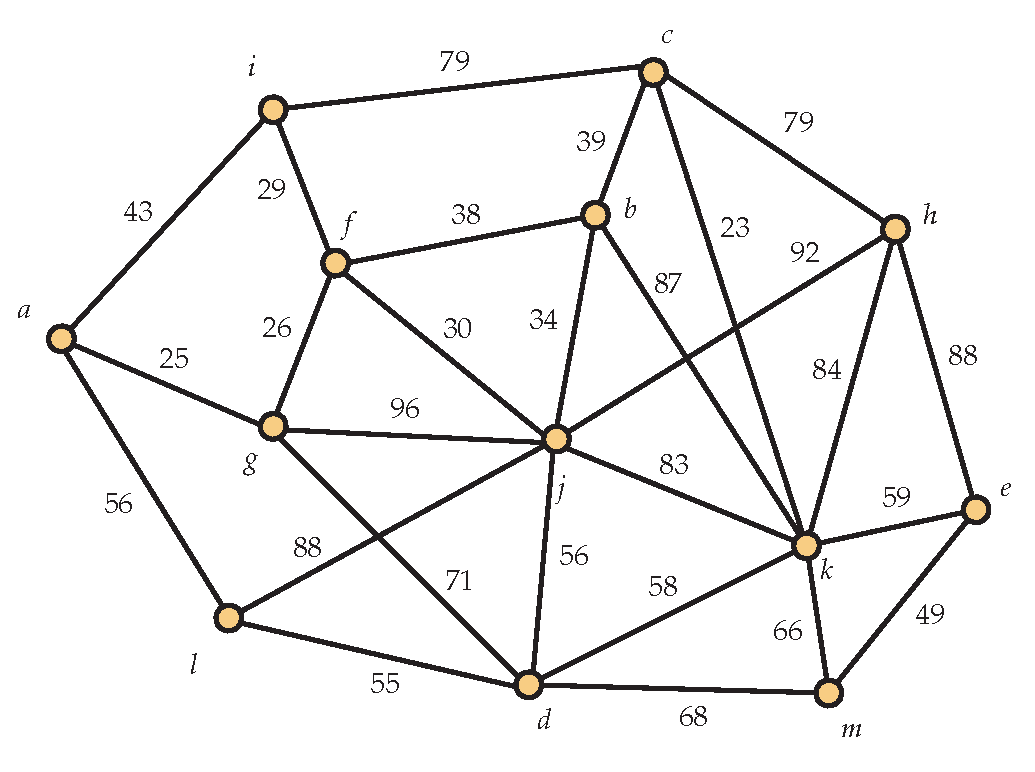
\includegraphics[width=3.5in]{graphalgorithms-figs/spantreegraph}
\caption{\label{fig:graphalgorithms:spantreegraph}A weighted graph}
\end{center}
\end{figure}
To do this, this section considers the following problem:
\begin{problem*}
   Find a minimum weight spanning tree $\bfT$ of $\bfG$.
\end{problem*}
To solve this problem, we will develop \textit{two} efficient graph
algorithms, each having certain computational advantages and
disadvantages. Before developing the algorithms, we need to establish
some preliminaries about spanning trees and forests.

\subsection{Preliminaries}

The following proposition about the number of components in a spanning
forest of a graph $\bfG$ has an easy inductive proof. You are asked to
provide it in the exercises.

\begin{proposition}\label{prop:graphalgorithms:spanforest}
Let $\GVE$ be a graph on $n$ vertices, and let $\bfH=(V,S)$ be
a spanning forest.  Then $0\le |S|\le n-1$.  Futhermore, if
$|S|= n-k$, then $\bfH$ has $k$ components.  In particular, $\bfH$ is
a spanning tree if and only if it contains $n-1$ edges.
\end{proposition}

The following proposition establishes a way to take a spanning tree of
a graph, remove an edge from it, and add an edge of the graph that is
not in the spanning tree to create a new spanning tree. Effectively,
the process exchanges two edges to form the new spanning tree, so we
call this the \emph{exchange principle}.

\begin{proposition}[Exchange Principle]\label{prop:graphalgorithms:exchange}
Let $\bfT=(V,S)$ be spanning tree in a graph $\bfG$, and let $e=xy$ be
an edge of $\bfG$ which does not belong to $\bfT$.  Then
\begin{enumerate}
\item  There is a \emph{unique} path $P=(x_0,x_1,x_2,\dots,x_t)$
with (a)~$x=x_0$; (b)~$y=x_t$; and (c)~$x_ix_{i+1}\in S$ for each
$i=0,1,2,\dots,t-1$.
\item  For each $i=0,1,2,\dots,t-1$, let $f_i=x_ix_{i+1}$ and 
  then set \[S_i = \{e\}\cup\{g\in S: g\neq f_i\},\] i.e., we \emph{exchange}
edge $f_i$ for edge $e$. Then $\bfT_i=(V,S_i)$ is a spanning tree of $\bfG$.
\end{enumerate}
\end{proposition}

\begin{proof}
  For the first fact, it suffices to note that if there were more than
  one distinct path from $x$ to $y$ in $\bfT$, we would be able to
  find a cycle in $\bfT$. This is impossible since it is a tree. For
  the second, we refer to \autoref{fig:graphalgorithms:exchange}. The
  black and green edges in the graph shown at the left represent the
  spanning tree $\bfT$. Thus, $f$ lies on the unique path from $x$ to
  $y$ in $\bfT$ and $e=xy$ is an edge of $\bfG$ \emph{not} in
  $\bfT$. Adding $e$ to $\bfT$ creates a graph with a unique cycle,
  since $\bfT$ had a unique path from $x$ to $y$. Removing $f$ (which
  could be any edge $f_i$ of the path, as stated in the proposition)
  destroys this cycle. Thus $\bfT_i$ is an acyclic subgraph of $\bfG$
  with $n-1+1-1=n-1$ edges, so it is a spanning tree.
  \begin{figure}[h]
    \centering
    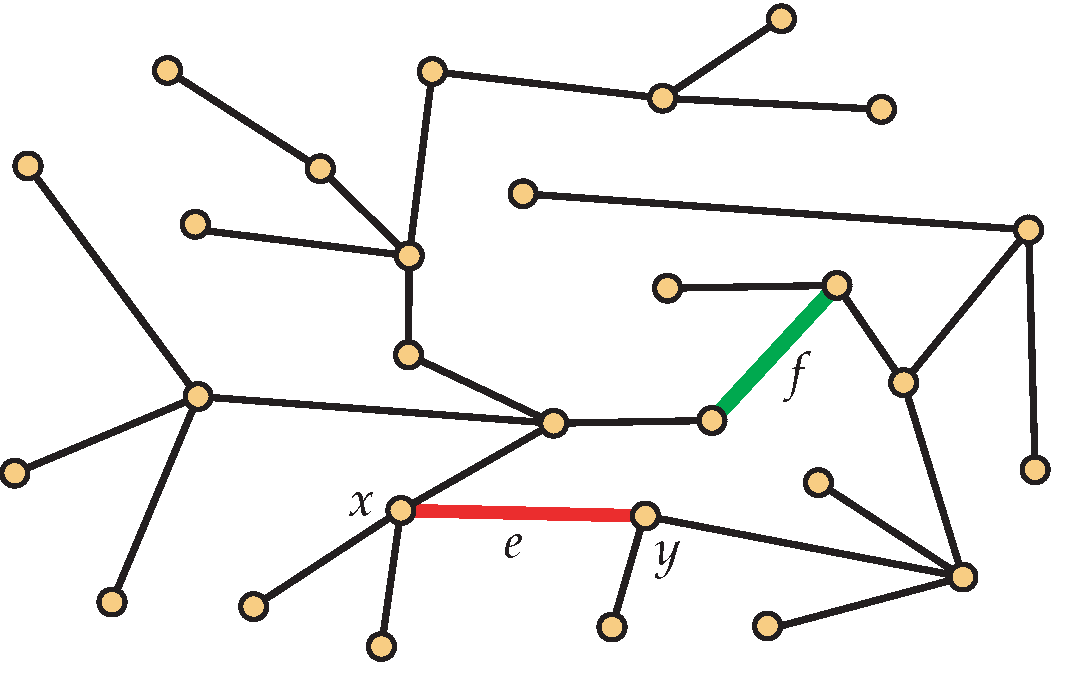
\includegraphics[width=0.45\linewidth]{graphalgorithms-figs/exchange1}\hspace{0.05\linewidth}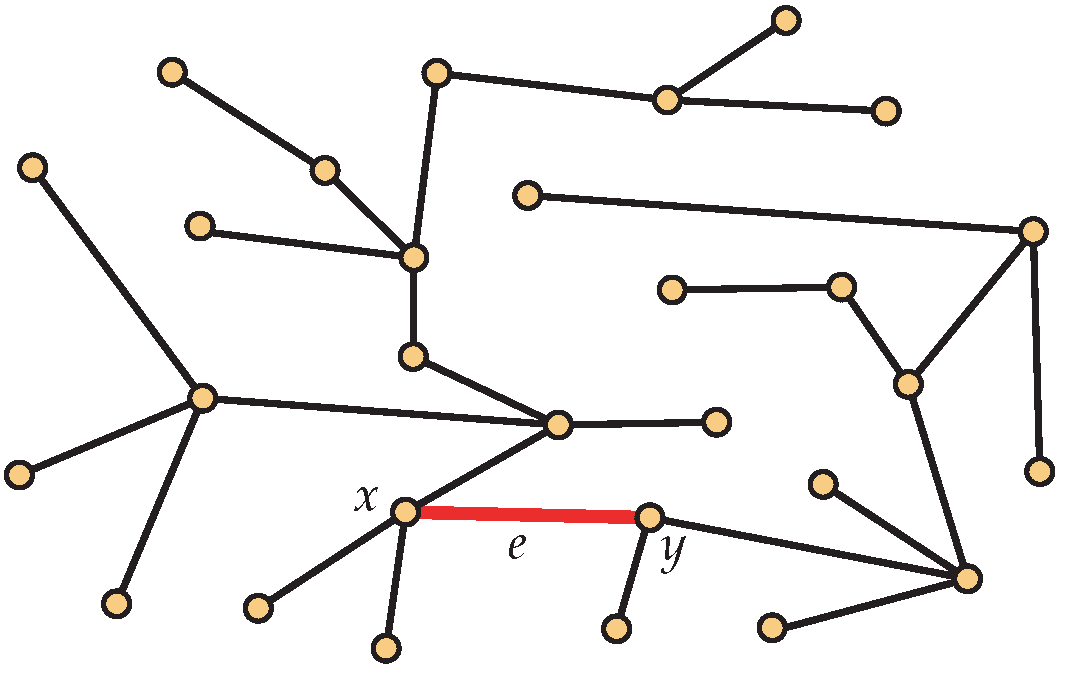
\includegraphics[width=0.45\linewidth]{graphalgorithms-figs/exchange2}
    \caption{The exchange principle}
    \label{fig:graphalgorithms:exchange}
  \end{figure}
\end{proof}
 
For both of the algorithms we develop, the argument to show that the
algorithm is optimal rests on the following technical lemma.  To avoid
trivialities, we assume $n\ge3$.

\begin{lemma}\label{lem:graphalgorithms:tech}
  Let $\bfF$ be a spanning forest of $\bfG$ and let $C$ be a component
  of $\bfF$.  Also, let $e=xy$ be an edge of minimum weight among all
  edges with one endpoint in $C$ and the other not in $C$.  Then among
  all spanning trees of $\bfG$ that contain the forest $\bfF$, there
  is one of minimum weight that contains the edge $e$.
\end{lemma}
\begin{proof}
  Let $\bfT=(V,S)$ be any spanning tree of minimum weight among all
  spanning trees that contain the forest $\bfF$, and suppose that
  $e=xy$ is not an edge in $\bfT$. (If it were an edge in $\bfT$, we
  would be done.) Then let $P=(x_0,x_1,x_2,\dots,x_t)$ be the unique
  path in $\bfT$ with (a)~$x=x_0$; (b)~$y=x_t$; and (c)~$x_ix_{i+1}\in
  S$ for each $i=0,1,2,\dots,t-1$.  Without loss of generality, we may
  assume that $x=x_0$ is a vertex in $C$ while $y=x_t$ does not
  belong to $C$.  Then there is a
  least non-negative integer $i$ for which $x_i$ is in $C$ and
  $x_{i+1}$ is not in $C$.  It follows that $x_j$ is in $C$ for all $j$ with
  $0\le j\le i$.

  Let $f=x_ix_{i+1}$. The edge $e$ has minimum weight among all edges
  with one endpoint in $C$ and the other not in $C$, so $w(e)\le
  w(f)$.  Now let $\bfT_i$ be the tree obtained by exchanging the edge
  $f$ for edge~$e$.  It follows that $w(\bfT_i) = w(\bfT) - w(f)
  +w(e)\le w(\bfT)$.  Furthermore, $\bfT_i$ contains the spanning
  forest $\bfF$ as well as the edge~$e$. It is therefore the minimum
  weight spanning tree we seek.
\end{proof}

\section{Discussion}
  Although Bob's combinatorial intuition has improved over the course
  he doesn't quite understand why we need
  special algorithms to find minimum weight spanning trees. He figures
  there can't be that many spanning trees, so he wants to just write
  them down. Alice groans as she senses that Bob must have
  been absent when the material from 
  \autoref{s:graphs:counting-trees}  was discussed.  In that section,
  we learned that a graph on $n$ vertices can have as many as $n^{n-2}$
  spanning trees (or horrors, the instructor may have left it off the
  syllabus).  Regardless, this exhaustive approach is already unusable
  when $n = 20$. Dave mumbles something about being greedy and just adding the
  lightest edges one-by-one while never adding an edge that would make
  a cycle. Zori remembers a strategy like this working for finding
  the height of a poset, but she's worried about the nightmare
  situation that we learned about with using FirstFit to color
  graphs. Alice agrees that greedy algorithms have an inconsistent
  track record but suggests that
  \hyperref[lem:graphalgorithms:tech]{Lemma~\ref*{lem:graphalgorithms:tech}}
  may be enough to get one to succeed here.

\subsection{Kruskal's Algorithm}

In this secton, we develop one of the best known algorithms for
finding a minimum weight spanning tree.  It is known as Kruskal's
Algorithm, although some prefer the descriptive label \textit{Avoid
  Cycles} because of the way it builds the spanning tree.

To start Kruskal's algorithm, we sort the edges according to weight.
To be more precise, let $m$ denote the number of edges in $\GVE$.
Then label the edges as $e_1,e_2,e_3,\dots,e_m$ so that $w(e_1)\le
w(e_2)\le \dots \le w(e_m)$. Any of the many available efficient
sorting algorithms can be used to do this step.

Once the edges are sorted, Kruskal's algorithm proceeds to an
initialization step and then inductively builds the spanning tree
$\bfT=(V,S)$:

\medskip
\textbf{Initialization.}\quad
Set $S=\emptyset$ and $i=0$.

\medskip
\textbf{Inductive Step.}\quad
While $|S| < n-1$, let $j$ be the least non-negative
integer so that $j > i$ and there are no cycles in
$S\cup\{e_j\}$.  Then (using pseudo-code) set
\[
i = j\quad\text{and}\quad S= S\cup\{j\}.
\]

The correctness of Kruskal's Algorithm follows from an inductive
argument. First, the set $S$ is initialized as the empty set, so there
is certainly a minimum weight spanning tree containing all the edges
in $S$.  Now suppose that for some $i$ with $0\le i <n$, $|S|=i$ and
there is a minimum weight spanning tree containing all the edges in
$S$.  Let $\bfF$ be the spanning forest determined by the edges in
$S$, and let $C_1, C_2,\dots,C_s$ be the components of $\bfF$.  For
each $k=1,2,\dots,s$, let $f_k$ be a minimum weight edge with one
endpoint in $C_k$ and the other not in $C_k$.  Then the edge $e$ added
to $S$ by Kruskal's Algorithm is just the edge $\{f_1,f_2,\dots,f_s\}$
having minimum weight. Applying
\hyperref[lem:graphalgorithms:tech]{Lemma~\ref*{lem:graphalgorithms:tech}}
and the inductive hypothesis, we know that there will still be a
minimum weight spanning tree of $\bfG$ containing all the edges of
$S\cup\{e\}$.

\medskip
\noindent\begin{minipage}{0.70\textwidth}
\begin{example}
  Let's see what Kruskal's algorithm does on the weighted graph in
  \autoref{fig:graphalgorithms:spantreegraph}. It first sorts all of
  the edges by weight. We won't reproduce the list here, since we
  won't need all of it. The edge of least weight is $ck$, which has
  weight $23$. It continues adding the edge of least weight, adding
  $ag$, $fg$, $fi$, $fj$, and $bj$. However, after doing this, the
  edge of lowest weight is $fb$, which has weight $38$. This edge
  cannot be added, as doing so would make $fjb$ a cycle. Thus, the
  algorithm bypasses it and adds $bc$. Edge $ai$ is next inspected,
  but it, too, would create a cycle and is eliminated from
  consideration. Then $em$ is added, followed by $dl$. There are now
  \emph{two} edges of weight $56$ to be considered: $al$ and $dj$. Our
  sorting algorithm has somehow decided one of them should appear
  first, so let's say it's $dj$. After adding $dj$, we cannot add
  $al$, as $agfjdl$ would form a cycle. Edge $dk$ is next considered,
  but it would also form a cycle. However, $ek$ can be added. Edges
  $km$ and $dm$ are then bypassed. Finally, edge $ch$ is added as the
  twelfth and final edge for this $13$-vertex spanning tree. The full
  list of edges added (in order) is shown to the right. The total
  weight of this spanning tree is $504$.\end{example}
\end{minipage}\hspace{.03\textwidth}
\begin{minipage}{.25\textwidth}
\begin{center}\textbf{Kruskal's Algorithm}\\%
  \begin{tt}c k 23\\%
     a g 25\\%
     f g 26\\%
     f i 29\\%
     f j 30\\%
     b j 34\\%
     b c 39\\%
     e m 49\\%
     d l 55\\%
     d j 56\\%
     e k 59\\%
     c h 79\end{tt}\end{center}\end{minipage}
\subsection{Prim's Algorithm}

We now develop Prim's Algorithm for finding a minimum weight spanning
tree. This algorithm is also known by a more descriptive label:
\textit{Build Tree}.  We begin by choosing a root vertex $r$. Again,
the algorithm proceeds with an initialization step followed by a
series of inductive steps.

\medskip
\textbf{Initialization.}\quad
Set $W=\{r\}$ and $S=\emptyset$.

\medskip
\textbf{Inductive Step.}\quad
While $|W| < n$, let $e$ be an edge of minimum weight among
all edges with one endpoint in $W$ and the other not in $W$.
If $e=xy$, $x\in W$ and $y\not\in W$, update $W$ and $S$ by
setting (using pseudo-code)
\[
W = W\cup\{y\}\quad\text{and}\quad S = S\cup\{e\}.
\]

The correctness of Prim's algorithm follows immediately from
\hyperref[lem:graphalgorithms:tech]{Lemma~\ref*{lem:graphalgorithms:tech}}.

\medskip
\noindent\begin{minipage}{0.70\textwidth}
\begin{example}
  Let's see what Prim's algorithm does on the weighted graph in
  \autoref{fig:graphalgorithms:spantreegraph}. We start with vertex
  $a$ as the root vertex. The lightest edge connecting $a$ (the only
  vertex in the tree so far) to the rest of the graph is $ag$. Next,
  $fg$ is added. This is followed by $fi$, $fj$, $bj$, and $bc$. Next,
  the algorithm identifies $ck$ as the lightest edge connecting
  $\{a,g,i,f,j,b,c\}$ to the remaining vertices. Notice that this is
  considerably later than Kruskal's algorithm finds the same edge. The
  algorithm then determines that $al$ and $jd$, both of weight $56$
  are the lightest edges connecting vertices in the tree to the other
  vertices. It picks arbitrarily, so let's say it takes $al$. It next
  finds $dl$, then $ek$, and then $em$. The final edge added is $ch$. The full
  list of edges added (in order) is shown to the right. The total
  weight of this spanning tree is $504$. This (not surprisingly) the
  same weight we obtained using Kruskal's algorithm. However, notice
  that the spanning tree found is different, as this one contains
  $al$ instead of $dj$. This is not an issue, of course, since in
  both cases an arbitrary choice between two edges of equal weight
  was made.\end{example}
\end{minipage}\hspace{.03\textwidth}
\begin{minipage}{.25\textwidth}
\begin{center}\textbf{Prim's Algorithm}\\

\medskip
\begin{tt}
a g 25\\
f g 26\\
f i 29\\
f j 30\\
b j 34\\
b c 39\\
c k 23\\
a l 56\\
d l 55\\
e k 59\\
e m 49\\
c h 79
\end{tt}\end{center}\end{minipage}

\subsection{Comments on Efficiency}

An implementation of Kruskal's algorithm seems to require that
the edges be sorted.  If the graph has $n$ vertices and $m$  edges,
this requires $m\log m$ operations just for the sort.  But once
the sort is done, the process takes only $n-1$ steps---provided
you keep track of the components as the spanning forest expands.
Regardless, it is easy to see that at most $O(n^2\log n)$ operations
are required.

On the other hand, an implementation of Prim's algorithm requires
the program to conveniently keep track of the edges incident with
each vertex and always be able to identify the edge with least
weight among subsets of these edges.  In computer science, the
data structure that enables this task to be carried out is called
a \textit{heap}.

\section{Digraphs}

In this section, we introduce another useful variant of a graph. In a
graph, the existence of an edge $xy$ can be used to model a connection
between $x$ and $y$ that goes in both ways. However, sometimes such a
model is insufficient. For instance, perhaps it is possible to fly
from Atlanta directly to Fargo but not possible to fly from Fargo
directly to Atlanta. In a graph representing the airline network, an
edge between Atlanta and Fargo would lose the information that the
flights only operate in one direction. To deal with this problem, we
introduce a new discrete structure. A \textit{digraph} $\bfG$ is a
pair $(V,E)$ where $V$ is a vertex set and $E\subset V\times V$ with
$x\neq y$ for every $(x,y)\in E$.  We consider the pair $(x,y)$ as a
\textit{directed edge} from $x$ to $y$.  Note that for distinct
vertices $x$ and $y$ from $V$, the ordered pairs $(x,y)$ and $(y,x)$
are distinct, so the digraph may have one, both or neither of the
directed edges $(x,y)$ and $(y,x)$. This is in contrast to graphs,
where edges are sets, so $\{x,y\}$ and $\{y,x\}$ are the same.

Diagrams of digraphs use arrowheads on the edges to indicate direction.
This is illustrated in \autoref{fig:graphalgorithms:digraph}. For
example, the digraph illustrated there contains the edge $(a,f)$ but
not the edge $(f,a)$. It does contain both edges $(c,d)$ and $(d,c)$,
however.

\begin{figure}[t]
\begin{center}
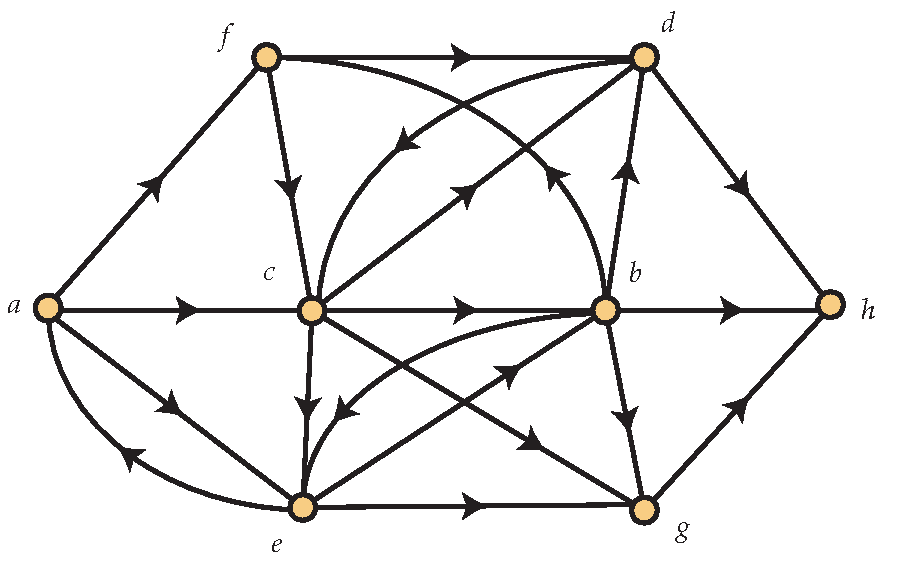
\includegraphics[width=3in]{graphalgorithms-figs/digraph}\\
\caption{A Digraph}
\label{fig:graphalgorithms:digraph}
\end{center}
\end{figure}

When $\bfG$ is a digraph, a sequence $P=(r=u_0,u_1,\dots,u_t=x)$ of
distinct vertices is called a \textit{directed path} from $r$ to $x$
when $(u_iu_{i+1})$ is a directed edge in $\bfG$ for every
$i=0,1,\dots,t-1$.  A directed path $C=(r=u_0,u_1,\dots,u_t=x)$ is
called a \textit{directed cycle} when $(u_t,u_0)$ is a directed edge
of $\bfG$.

\section{Dijkstra's Algorithm for Shortest Paths}

Just as with graphs, it is useful to assign weights to the directed
edges of a digraph. Specifically, in this section we consider a pair
$(\bfG,w)$ where $\GVE$ is a digraph and $w:E\rightarrow\mathbb{N}_0$
is a function assigning to each directed edge $(x,y)$ a non-negative
weight $w(x,y)$.  However, in this section, we interpret weight as
\textit{distance} so that $w(x,y)$ is now called the \textit{length}
of the edge $(x,y)$.  If $P=(r=u_0,u_1,\dots,u_t=x)$ is a directed
path from $r$ to $x$, then the \textit{length} of the path $P$ is just
the sum of the lengths of the edges in the path, $\sum_{i=0}^{t-1}
w(u_iu_{i+1})$.  The \textit{distance} from $r$ to $x$ is then defined
to be the minimum length of a directed path from $r$ to $x$. Our goal
in this section is to solve the following natural problem, which has
many applications:

\medskip
\noindent\textbf{Problem.}\quad
For each vertex $x$, find the distance from $r$ to $x$.  Also, find a
shortest path from $r$ to $x$.

\subsection{Description of the Algorithm}

To describe Dijkstra's algorithm in a compact manner, it is useful to
extend the definition of the function $w$. We do this by by setting
$w(x,y)=\infty$ when $x\neq y$ and $(x,y)$ is not a directed edge of
$\bfG$. In this way, we will treat $\infty$ as if it were a number
(although it is not!).\footnote{This is not an issue for computer
  implementation of the algorithm, as instead of using $\infty$, a
  value given by the product of the number of vertices and the 
  maximum edge weight may be used to simulate infinity.} 

Let $n=|V|$.  At Step~$i$, where $1\le i\le n$, we will 
have determined: 
\begin{enumerate}
\item A sequence $\sigma=(v_1,v_2,v_3,\dots,v_i)$ of distinct 
vertices from $\bfG$ with $r=v_1$.  These vertices are called 
\textit{permanent} vertices, while the remaining vertices will
be called \textit{temporary} vertices.
\item For each vertex $x\in V$, we will have determined a
  number $\delta(x)$ and a path $P(x)$ from $r$ to $x$ of
  length $\delta(x)$.
\end{enumerate}

\noindent\textbf{Initialization} (Step 1).\quad
Set $i=1$. Set $\delta(r)=0$ and let $P(r)=(r)$ be the trivial
one-point path.  Also, set $\sigma= (r)$.  For each $x\neq r$, set
$\delta(x)= w(r,x)$ and $P(x)=(r,x)$. Let $x$ be a temporary vertex
for which $\delta(x)$ is minimum. Set $v_2 = x$, and update $\sigma$
by appending $v_2$ to the end of it. Increment $i$.

\medskip
\noindent\textbf{Inductive Step} (Step $i$, $i>1$).\quad
If $i<n$, then
for each temporary $x$, let
\[\delta(x) = \min\{\delta(x), \delta(v_i)+w(v_i,x)\}.\]
If this assignment results in a reduction in the
value of $\delta(x)$, let $P(x)$ be the
path obtained by adding $x$ to the end of $P(v_i)$.

Let $x$ be a temporary vertex for which $\delta(x)$ is minimum.  Set
$v_{i+1}=x$, and update $\sigma$ by appending $v_{i+1}$ to
it. Increment $i$.

\subsection{Example}

Before establishing why Dijkstra's algorithm works, it may be helpful
to see an example of how it works. To do this, consider the digraph
$\bfG$ shown in \autoref{fig:graphalgorithms:dijkstragraph}.  For
visual clarity, we have chosen a digraph which is an \textit{oriented
  graph}, i.e., for each distinct pair $x,y$ of vertices, the graph
contains at most one of the two possible directed edges $(x,y)$ and
$(y,x)$.

\begin{figure}[t]
\begin{center}
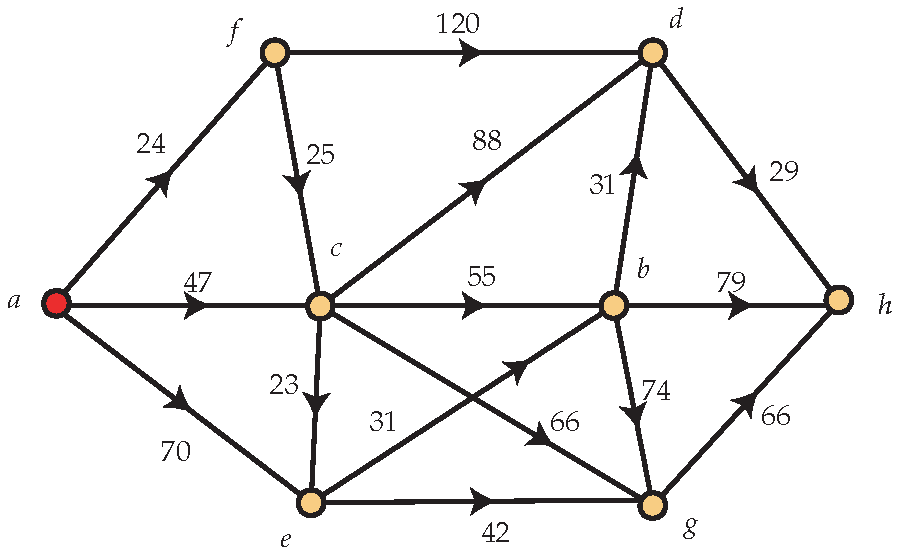
\includegraphics[width=3in]{graphalgorithms-figs/dijkstragraph}\\
\caption{A digraph with edge lengths}
\label{fig:graphalgorithms:dijkstragraph}
\end{center}
\end{figure}

Suppose that the root vertex $r$ is the vertex labeled~$a$. The
initialization step of Dijkstra's algorithm then results in the
following values for $\delta$ and $P$:

\textbf{Initialization (Step 1)}

\begingroup
\leftskip25pt
\rightskip\leftskip

\medskip
$\sigma=(a)$\\
$\delta(a)=0$; $P(a)=(a)$\\
$\delta(b)=\infty$; $P(b)=(a,b)$\\
$\delta(c)=47$; $P(c)=(a,c)$\\
$\delta(d)=\infty$; $P(d)=(a,d)$\\
$\delta(e)=70$; $P(e)=(a,e)$\\
$\delta(f)=24$; $P(f)=(a,f)$\\
$\delta(g)=\infty$; $P(g)=(a,g)$\\
$\delta(h)=\infty$; $P(h)=(a,h)$\\

\endgroup

Before finishing Step 1, the algorithm identifies vertex~$f$ as
closest to $a$ and appends it to $\sigma$, making $a$ permanent. When
entering Step 2, Dijkstra's algorithm attempts to find shorter paths
from $a$ to each of the temporary vertices by going through $f$. We
call this process ``scanning from vertex~$f$.'' In this scan, the path
to vertex~$d$ is updated, since $\delta(f) + w(f,d)=24+120=144<
\infty=w(a,d)$.

\medskip
\textbf{Step 2.}\quad Scan from vertex~$f$.

\begingroup
\leftskip25pt
\rightskip\leftskip

\medskip
$\sigma=(a,f)$\\
$\delta(a)=0$; $P(a)=(a)$\\
$\delta(b)=\infty$; $P(b)=(a,b)$\\
$\delta(c)=47$; $P(c)=(a,c)$\\
$\delta(d)=144 = 24 + 120 = \delta(f)+w(f,d)$; $P(d)=(a,f,d)$\quad\text{updated}\\
$\delta(e)=70$; $P(e)=(a,e)$\\
$\delta(f)=24$; $P(f)=(a,f)$\\
$\delta(g)=\infty$; $P(g)=(a,f)$\\
$\delta(h)=\infty$; $P(h)=(a,h)$\\

\endgroup

Before proceeding to the next step, vertex~$c$ is made permanent by
making it $v_3$. In Step 3, therefore, the scan is from vertex
$c$. Vertices $b$, $d$, and $g$ have their paths updated. However,
although $\delta(c) + w(c,e) = 47+23=70=\delta(e)$, we do not
change $P(e)$ since $\delta(e)$ is not \emph{decreased} by routing
$P(e)$ through $c$.

\medskip
\textbf{Step 3.}\quad Scan from vertex~$c$.

\begingroup
\leftskip25pt
\rightskip\leftskip

\medskip
$\sigma=(a,f,c)$\\
$\delta(a)=0$; $P(a)=(a)$\\
$\delta(b)=102=47+55= \delta(c)+w(c,b)$; $P(b)=(a,c,b)$\quad\text{updated}\\
$\delta(c)=47$; $P(c)=(a,c)$\\
$\delta(d)=135=47+88 = \delta(c)+w(c,d)$; $P(d)=(a,c,d)$\quad\text{updated}\\
$\delta(e)=70$; $P(e)=(a,e)$\\
$\delta(f)=24$; $P(f)=(a,f)$\\
$\delta(g)=113=47+66= \delta(c)+w(c,g)$; $P(g)=(a,c,g)$\quad\text{updated}\\
$\delta(h)=\infty$; $P(h)=(a,h)$\\

\endgroup

Now vertex $e$ is made permanent.

\medskip
\textbf{Step 4.}\quad Scan from vertex~$e$.

\begingroup
\leftskip25pt
\rightskip\leftskip

\medskip
$\sigma=(a,f,c,e)$\\
$\delta(a)=0$; $P(a)=(a)$\\
$\delta(b)=101=70+31= \delta(e)+w(e,b)$; $P(b)=(a,e,b)$\quad\text{updated}\\
$\delta(c)=47$; $P(c)=(a,c)$\\
$\delta(d)=135$; $P(d)=(a,c,d)$\\
$\delta(e)=70$; $P(e)=(a,e)$\\
$\delta(f)=24$; $P(f)=(a,f)$\\
$\delta(g)=112=70+42= \delta(e)+w(e,g)$; $P(g)=(a,e,g)$\quad\text{updated}\\
$\delta(h)=\infty$; $P(h)=(a,h)$\\

\endgroup

Now vertex $b$ is made permanent.

\medskip
\textbf{Step 5.}\quad Scan from vertex~$b$.

\begingroup
\leftskip25pt
\rightskip\leftskip

\medskip
$\sigma=(a,f,c,e,b)$\\
$\delta(a)=0$; $P(a)=(a)$\\
$\delta(b)=101$; $P(b)=(a,e,b)$\\
$\delta(c)=47$; $P(c)=(a,c)$\\
$\delta(d)= 132 = 101+ 31= \delta(b)+w(b,d)$; $P(d)=(a,e,b,d)$\quad\text{updated}\\
$\delta(e)= 70$; $P(e)=(a,e)$\\
$\delta(f)= 24$; $P(f)=(a,f)$\\
$\delta(g)=112$; $P(g)=(a,e,g)$\\
$\delta(h)=180 = 101+79=\delta(b)+w(b,h)$; $P(h)=(a,e,b,h)$\quad\text{updated}\\

\endgroup

Now vertex $g$ is made permanent.

\medskip
\textbf{Step 6.}\quad Scan from vertex~$g$.

\begingroup
\leftskip25pt
\rightskip\leftskip

\medskip
$\sigma=(a,f,c,e,b,g)$\\
$\delta(a)=0$; $P(a)=(a)$\\
$\delta(b)=101$; $P(b)=(a,e,b)$\\
$\delta(c)=47$; $P(c)=(a,c)$\\
$\delta(d)= 132$; $P(d)=(a,e,b,d)$\\
$\delta(e)=70$; $P(e)=(a,e)$\\
$\delta(f)=24$; $P(f)=(a,f)$\\
$\delta(g)=112$; $P(g)=(a,e,g)$\\
$\delta(h)=178 = 112+66=\delta(g)+w(g,h)$; $P(h)=(a,e,g,h)$\quad\text{updated}\\

\endgroup

Now vertex $d$ is made permanent.

\medskip
\textbf{Step 7.}\quad Scan from vertex~$d$.

\begingroup
\leftskip25pt
\rightskip\leftskip

\medskip
$\sigma=(a,f,c,e,b,g,d)$\\
$\delta(a)=0$; $P(a)=(a)$\\
$\delta(b)=101$; $P(b)=(a,e,b)$\\
$\delta(c)=47$; $P(c)=(a,c)$\\
$\delta(d)= 132$; $P(d)=(a,e,b,d)$\\
$\delta(e)=70$; $P(e)=(a,e)$\\
$\delta(f)=24$; $P(f)=(a,f)$\\
$\delta(g)=112$; $P(g)=(a,e,g)$\\
$\delta(h)=161 = 132+29=\delta(d)+w(d,h)$; $P(h)=(a,e,b,d,h)$\quad\text{updated}\\

\endgroup

Now vertex $h$ is made permanent. Since this is the last vertex, the
algorithm halts and returns the following:

\medskip
\textbf{FINAL RESULTS}\quad 

\begingroup
\leftskip25pt
\rightskip\leftskip

\medskip
$\sigma=(a,f,c,e,b,g,d,h)$\\
$\delta(a)=0$; $P(a)=(a)$\\
$\delta(b)=101$; $P(b)=(a,e,b)$\\
$\delta(c)=47$; $P(c)=(a,c)$\\
$\delta(d)= 132$; $P(d)=(a,e,b,d)$\\
$\delta(e)=70$; $P(e)=(a,e)$\\
$\delta(f)=24$; $P(f)=(a,f)$\\
$\delta(g)=112$; $P(g)=(a,e,g)$\\
$\delta(h)=161$; $P(h)=(a,e,b,d,h)$\\

\endgroup

\subsection{The Correctness of Dijkstra's Algorithm}

Now that we've illustrated Dijkstra's algorithm, it's time to prove
that it actually does what we claimed it does: find the distance from
the root vertex to each of the other vertices and a path of that
length. To do this, we first state two elementary propositions. The
first is about shortest paths in general, while the second is specific
to the sequence of permanent vertices produced by Dijkstra's algorithm.

\begin{proposition}
Let $x$ be a vertex and let $P=(r=u_0,u_1,\dots,u_t=x)$ be
a shortest path from $r$ to $x$.  Then for every
integer $j$ with $0<j<t$,
$(u_0,u_1,\dots,u_j)$ is a shortest path from $r$
to $u_j$ and $(u_j,u_{j+1},\dots,u_t)$ is a shortest
path from $u_j$ to $u_t$
\end{proposition}

\begin{proposition}
When the algorithm halts, let $\sigma=(v_1,v_2,v_3,\dots,v_n)$. 
Then \[\delta(v_1)\le \delta(v_2)\le\dots \le \delta(v_n). \]
\end{proposition}

We are now ready to prove the correctness of the algorithm. The proof
we give will be inductive, but the induction will have nothing to do
with the total number of vertices in the digraph or the step number
the algorithm is in.

\begin{theorem}
  Dijkstra's algorithm yields shortest paths for every vertex $x$ in
  $\bfG$. That is, when Dijkstra's algorithm terminates, for each
  $x\in V$, the value $\delta(x)$ is the distance from $r$ to $x$ and
  $P(x)$ is a shortest path from $r$ to $x$.
\end{theorem}

\begin{proof}
  The theorem holds trivially when $x=r$.  So we consider the case
  where $x\neq r$.  We argue that $\delta(x)$ is the distance from $r$
  to $x$ and that $P(x)$ is a shortest path from $r$ to $x$ by
  induction on the minimum number $k$ of edges in a shortest path from
  $r$ to $x$. When $k=1$, the edge $(r,x)$ is a shortest path from $r$
  to $x$.  Since $v_1=r$, we will set $\delta(x)=w(r,x)$ and
  $P(x)=(r,x)$ at Step~1.

  Now fix a positive integer $k$. Assume that if the minimum number of
  edges in a shortest path from $r$ to $x$ is at most $k$, then
  $\delta(x)$ is the distance from $r$ to $x$ and $P(x)$ is a shortest
  path from $r$ to $x$. Let $x$ be a vertex for which the minimum
  number of edges in a shortest path from $r$ to $x$ is $k+1$.  Fix a
  a shortest path $P=(u_0,u_1,u_2,\dots,u_{k+1})$ from $r=u_0$ to
  $x=u_{k+1}$.  Then $Q=(u_0,u_1,\dots,u_k)$ is a shortest path from
  $r$ to $u_k$. (See \autoref{fig:graphalgorithms:dijkstra-proof}.)

  \begin{figure}[b]
    \centering
    \begin{overpic}[width=0.6\textwidth]{graphalgorithms-figs/dijkstra-proof}
      \put(3,13){$r$}
      \put(33,25){$Q$}
      \put(58,3){$P(u_k)$}
      \put(73,28){$u_k$}
      \put(83,25){$P$}
      \put(93,21){$x$}
    \end{overpic}
    \caption{Shortest paths}
    \label{fig:graphalgorithms:dijkstra-proof}
  \end{figure}

  By the inductive hypothesis, $\delta(u_k)$ is the distance from $r$
  to $u_k$, and $P(u_k)$ is a shortest path from $r$ to $u_k$.  Note
  that $P(u_k)$ need not be the same as path $Q$, as we suggest in
  \autoref{fig:graphalgorithms:dijkstra-proof}.  However, if distinct,
  the two paths will have the same length, namely $\delta(u_k)$.
  Also, the distance from $r$ to $x$ is $\delta(u_k)+w(u_k,x)\ge
  \delta(u_k)$ since $P$ is a shortest path from $r$ to $x$ and
  $w(u_k,x)\geq 0$.

  Let $i$ and $j$ be the unique integers for which $u_k=v_i$ and
  $x=v_j$.  If $j < i$, then
  \[
  \delta(x)= \delta(v_j)\le \delta(v_i)= \delta(u_k)\le
  \delta(u_k)+w(u_k).
  \]
  Therefore the algorithm has found a path $P(x)$ from $r$ to $x$
  having length $\delta(x)$ which is at most the distance from $r$ to
  $x$.  Clearly, this implies that $\delta(x)$ is the distance from
  $r$ to $x$ and that $P(x)$ is a shortest path.

  On the other hand, if $j>i$, then the inductive step at Step~$i$
  results in
  \[
  \delta(x)\le \delta(v_i)+w(v_i,y)=\delta(u_k)+w(u_k,x).
  \]
  As before, this implies that $\delta(x)$ is the distance from $r$ to
  $x$ and that $P(x)$ is a shortest path.
\end{proof}


\section{Historical Notes}

Kruskal's algorithm was published in 1956 by Joseph B.\ Kruskal in a
three-page paper that appeared in \emph{Proceedings of the American
  Mathematical Society}. Robert C.\ Prim published the algorithm that
now bears his name the following year in \emph{The Bell System
  Technical Journal}. Prim's paper focuses on application of the
minimum weight (or length or cost) spanning tree problem to telephone
networks. He was aware of Kruskal's prior work, as they were
colleagues at Bell Laboratories at the time he published his paper. It
turns out that Prim had been beaten to the punch by Czech
mathematician Vojt\v{e}ch Jarn\'{i}k in 1929, so some refer to Prim's
algorithm as Jarn\'{i}k's algorithm. (It was later rediscovered by
Dijkstra, so some attach his name as well, referring to it as the
Dijkstra-Jarn\'{i}k-Prim algorithm.) Edsger Dijkstra published his
algorithm for finding shortest paths in 1959 in a three-page
paper\footnote{This is also the paper in which Prim's algorithm was
  published for the third time. Dijkstra was aware of Kruskal's prior
  work but argued that his algorithm was preferable because it
  required that less information about the graph be stored in memory
  at each step of the algorithm.}  appearing in \emph{Numerische
  Mathematik}. In fact, Dijkstra's algorithm had been discovered (in
an equivalent form) by Edward F.\ Moore two years earlier. His result
appeared in \emph{Proceedings of an International Symposium on the
  Theory of Switching}.

\section{Exercises}

\begin{enumerate}
\item For the graph in \autoref{fig:span_tree_ex1}, use Kruskal's
  algorithm (``avoid cycles'') to find a minimum weight spanning
  tree. Your answer should include a complete list of the edges,
  indicating which edges you take for your tree and which (if any) you
  reject in the course of running the algorithm.
  \begin{figure}[h]
    \centering
    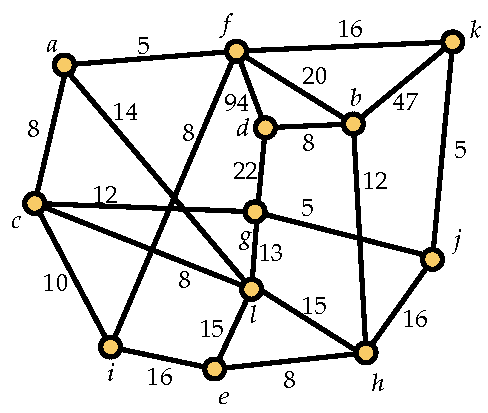
\includegraphics[scale=0.65]{graphalgorithms-figs/span_tree_ex1}
    \caption{Find a minimum weight spanning tree}
    \label{fig:span_tree_ex1}
  \end{figure}
\item For the graph in \autoref{fig:span_tree_ex1}, use Prim's
  algorithm (``build tree'') to find a minimum weight spanning
  tree. Your answer should list the edges selected by the algorithm in
  the order they were selected.
\item For the graph in \autoref{fig:span_tree_ex2}, use Kruskal's
  algorithm (``avoid cycles'') to find a minimum weight spanning
  tree. Your answer should include a complete list of the edges,
  indicating which edges you take for your tree and which (if any) you
  reject in the course of running the algorithm.
  \begin{figure}[h]
    \centering
    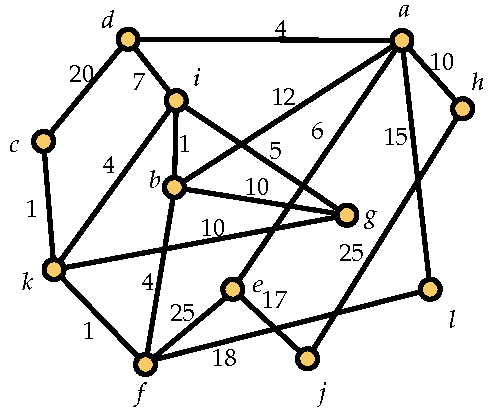
\includegraphics[scale=0.65]{graphalgorithms-figs/span_tree_ex2}
    \caption{Find a minimum weight spanning tree}
    \label{fig:span_tree_ex2}
  \end{figure}
\item For the graph in \autoref{fig:span_tree_ex2}, use Prim's
  algorithm (``build tree'') to find a minimum weight spanning
  tree. Your answer should list the edges selected by the algorithm in
  the order they were selected.
\item For the graph in \autoref{fig:span_tree_ex3}, use Kruskal's
  algorithm (``avoid cycles'') to find a minimum weight spanning
  tree. Your answer should include a complete list of the edges,
  indicating which edges you take for your tree and which (if any) you
  reject in the course of running the algorithm.
  \begin{figure}[h]
    \centering
    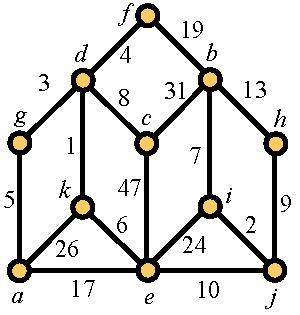
\includegraphics[scale=0.65]{graphalgorithms-figs/span_tree_ex3}
    \caption{Find a minimum weight spanning tree}
    \label{fig:span_tree_ex3}
  \end{figure}
\item For the graph in \autoref{fig:span_tree_ex3}, use Prim's
  algorithm (``build tree'') to find a minimum weight spanning
  tree. Your answer should list the edges selected by the algorithm in
  the order they were selected.
\item A new local bank is being created and will establish a
  headquarters $h$, two branches $b_1$ and $b_2$, and four ATMs $a_1$,
  $a_2$, $a_3$, and $a_4$. They need to build a computer network such
  that the headquarters, branches, and ATMs can all
  intercommunicate. Furthermore, they will need to be networked with
  the Federal Reserve Bank of Atlanta, $f$. The costs of the feasible
  network connections (in units of \$10,000) are listed below:
  \begin{align*}
    h f & \quad 80 &
    h b_1 & \quad 10\\
    h b_2 & \quad 20&
    b_1 b_2 & \quad 8\\
    f b_1 & \quad 12&
    f a_1 & \quad 20\\
    b_1 a_1 & \quad 3&
    a_1 a_2 & \quad 13\\
    h a_2 & \quad 6&
    b_2 a_2 & \quad 9\\
    b_2 a_3 & \quad 40&
    a_1 a_4 & \quad 3\\
    a_3 a_4 &\quad 6
  \end{align*}
  The bank wishes to minimize the cost of building its network (which
  must allow for connection, possibly routed through other nodes, from
  each node to each other node), however due to the need for
  high-speed communication, they \textbf{must} pay to build the
  connection from $h$ to $f$ as well as the connection from $b_2$ to
  $a_3$. Give a list of the connections the bank should establish in
  order to minimize their total cost, subject to this constraint. Be
  sure to explain how you selected the connections and how you know
  the total cost is minimized.
\item A disconnected weighted graph obviously has no spanning
  trees. However, it is possible to find a spanning forest of minimum
  weight in such a graph. Explain how to modify both Kruskal's
  algorithm and Prim's algorithm to do this.
\item Prove
  \hyperref[prop:graphalgorithms:spanforest]{Proposition~\ref*{prop:graphalgorithms:spanforest}}.
\item In the paper where Kruskal's algorithm first appeared, he
  considered the algorithm a route to a nicer proof that in a
  connected weighted graph with no two edges having the same weight,
  there is a \emph{unique} minimum weight spanning tree. Prove this
  fact using Kruskal's algorithm.
\item Use Dijkstra's algorithm to find the distance from $a$ to each
  other vertex in the digraph shown in
  \autoref{fig:graphalgorithms:dijkstra_ex1} and a directed path of
  that length.
  \begin{figure}[h]
    \centering
    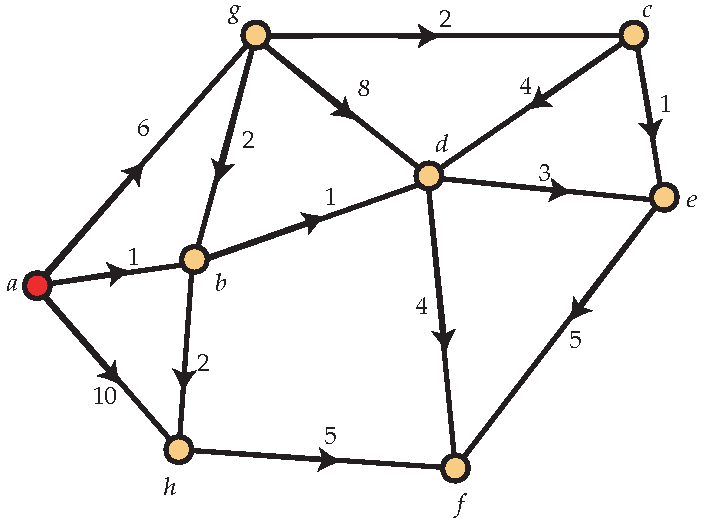
\includegraphics[scale=0.65]{graphalgorithms-figs/dijkstra_ex1}
    \caption{A directed graph}
    \label{fig:graphalgorithms:dijkstra_ex1}
  \end{figure} 

\begin{minipage}{0.5\textwidth}
\item The table to the right contains the length of the directed edge
  $(x,y)$ in the intersection of \textbf{row} $x$ and \textbf{column}
  $y$ in a digraph with vertex set $\{a,b,c,d,e,f\}$. For example,
  $w(b,d)=21$. (On the other hand, $w(d,b)=10$.) Use this data and
  Dijkstra's algorithm to find the distance from $a$ to each of the
  other vertices and a directed path of that length from $a$.
\end{minipage}\hspace{0.02\textwidth}\begin{minipage}{0.45\textwidth}
\begin{tabular}{|c|c|c|c|c|c|c|c|}
  \hline
  $w$ &  $a$ &  $b$ &  $c$ &  $d$ &  $e$ &  $f$ \\ \hline 
  $a$ &  0 & 12 & 8 & 43 & 79 & 35 \\ \hline 
  $b$ & 93 &  0 & 18 & 21 & 60 & 33  \\ \hline 
  $c$ & 17 & 3 &  0 & 37 & 50  & 30 \\ \hline 
  $d$ & 85 & 10 & 91 &  0 & 17  & 7 \\ \hline 
  $e$ & 28 & 47 & 39 & 14  &  0 & 108 \\ \hline 
  $f$ & 31 & 7  & 29 & 73 & 20 &  0 \\ \hline 
\end{tabular}
\end{minipage}

\item Use Dijkstra's algorithm to find the distance from $a$ to each
  other vertex in the digraph shown in
  \autoref{fig:graphalgorithms:dijkstra_ex2} and a directed path of
  that length.
  \begin{figure}[h]
    \centering
    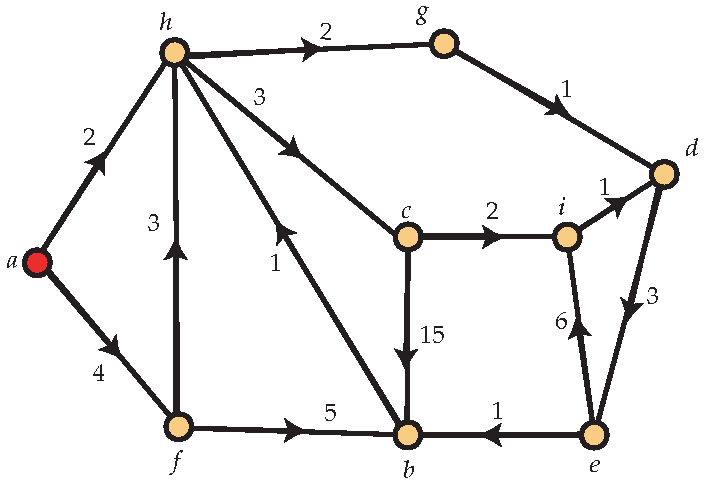
\includegraphics[scale=0.65]{graphalgorithms-figs/dijkstra_ex2}
    \caption{A directed graph}
    \label{fig:graphalgorithms:dijkstra_ex2}
  \end{figure}

\begin{minipage}{0.5\textwidth}
\item The table to the right contains the length of the directed edge
  $(x,y)$ in the intersection of \textbf{row} $x$ and \textbf{column}
  $y$ in a digraph with vertex set $\{a,b,c,d,e,f\}$. For example,
  $w(b,d)=47$. (On the other hand, $w(d,b)=6$.) Use this data and
  Dijkstra's algorithm to find the distance from $a$ to each of the
  other vertices and a directed path of that length from $a$.
\end{minipage}\hspace{0.02\textwidth}\begin{minipage}{0.45\textwidth}
    \begin{tabular}{|c|c|c|c|c|c|c|}
      \hline
      $w$ & $a$ & $b$ & $c$ & $d$ & $e$ & $f$\\
      \hline
      $a$ & 0 & 7 & 17 & 55 & 83 & 42\\
      \hline
      $b$ & 14 & 0 & 13 & 47 & 27 & 17\\
      \hline
      $c$ & 37 & 42 & 0 & 16 & 93 & 28\\
      \hline
      $d$ & 10 & 6 & 8 & 0 & 4 & 32\\
      \hline
      $e$ & 84 & 19 & 42 & 8 & 0 & 45\\
      \hline
      $f$ & 36 & 3 & 76 & 5 & 17 & 0\\
      \hline
    \end{tabular}
\end{minipage}

\item Give an example of a digraph having an \emph{undirected} path
  between each pair of vertices, but having a root vertex $r$ so that
  Dijkstra's algorithm cannot find a path of finite length from $r$ to some
  vertex $x$.
\item Notice that in our discussion of Dijkstra's algorithm, we
  required that the edge weights be nonnegative. If the edge weights
  are lengths and meant to model distance, this makes perfect
  sense. However, in some cases, it might be reasonable to allow
  negative edge weights. For example, suppose that a positive weight
  means there is a cost to travel along the directed edge while a
  negative edge weight means that you make money for traveling along
  the directed edge. In this case, a directed path with positive total
  weight results in paying out to travel it, while one with negative
  total weight results in a profit.
  \begin{enumerate}
  \item Give an example to show that Dijkstra's algorithm does not
    always find the path of minimum total weight when negative edge
    weights are allowed.
  \item Bob and Xing are considering this situation, and Bob suggests
    that a little modification to the algorithm should solve the
    problem. He says that if there are negative weights, they just
    have to find the smallest (i.e., most negative weight) and add the
    absolute value of that weight to every directed edge. For example, if
    $w(x,y)\geq -10$ for every directed edge $(x,y)$, Bob is
    suggesting that they add $10$ to every edge weight. Xing is
    skeptical, and for good reason. Give an example to show why Bob's
    modification won't work.
  \end{enumerate}


\end{enumerate}

%%% Local Variables: 
%%% mode: latex
%%% TeX-master: "chap-skel-mtk"
%%% End: 
